\documentclass[aspectratio=169,12pt]{beamer}
\usetheme[language=english]{ubbeamer2023}

\title{Hello \& Welcome!}
\subtitle{\href{https://www.ana.unibe.ch/weiterbildung/comulis_training_school/}{COMULIS Training School - Imaging Across Scales}}
\author{Ruslan Hlushchuk | Benoît Zuber | Yury Belyaev}
\institute{Institute of Anatomy}
\date{August 25, 2025}

\begin{document}

\begin{frame}
	\titlepage
\end{frame}

\begin{frame}{Wi-Fi}
	\begin{itemize}
		\item Either use \emph{\href{https://www.eduroam.org/}{eduroam}}
		\item Or connect your device to \emph{public-unibe}
		\begin{itemize}
			\item Select the menu item \emph{Guest Login}
			\item Enter your mobile number
			% Get the currently valid guest voucher here: https://serviceportal.unibe.ch/sp?id=kb_article_view&sysparm_article=KB0010178
			% Copy-paste it into the `voucher.tex` file, since "The voucher code must not be published publicly on the internet or other public places, rooms, pinboards or similar."
			% The GitHub Action (https://github.com/habi/Talk.2025.COMULIS/blob/bf06318c1d5e90722e36e62347770deda5f170c5/.github/workflows/latex.yaml#L23) gets the current secret as base64-encoded value via https://github.com/habi/Talk.2025.COMULIS/settings/secrets/actions as `VOUCHER_B64`
			\item Enter the voucher code \alert{\input{voucher.txt}}
			\item Access code is then provided by SMS
		\end{itemize}
	\end{itemize}
\end{frame}

\begin{frame}{Program}
	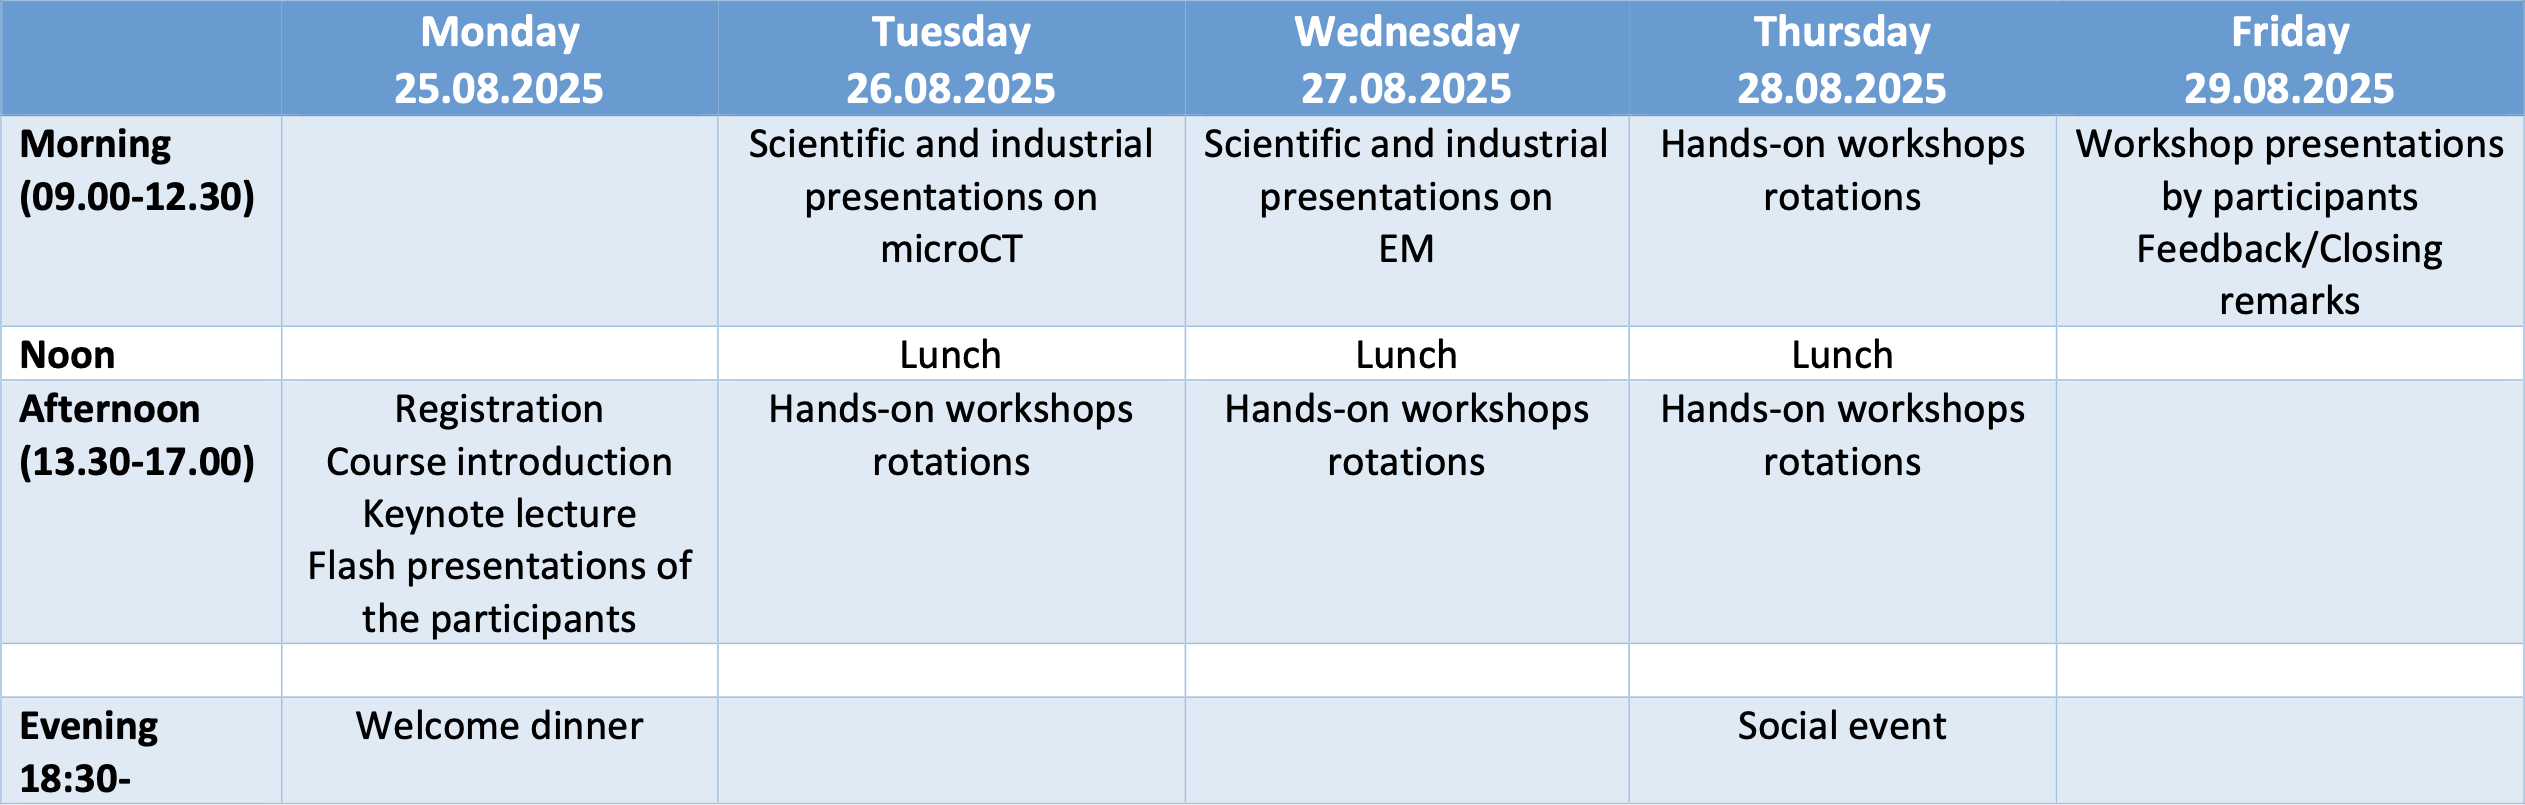
\includegraphics[width=\textwidth]{./images/program.png}
\end{frame}

\end{document}